\documentclass[10pt,letterpaper]{article}
\usepackage[utf8]{inputenc}
\usepackage[T1]{fontenc}
\usepackage[margin=0.6in]{geometry}
\usepackage{amsmath,amssymb,mathtools,graphicx,booktabs,xcolor,hyperref}
\setlength{\parindent}{0pt}
\setlength{\parskip}{5pt}
\begin{document}

\section*{Block S4 Solutions: DC-Driven Series RLC Circuit Analysis}

  \textbf{Companion Key to:} \texttt{Block\_S4\_Exercises\_DC\_RLC\_Circuits.pdf} ~|~
  \textbf{Verification:} Cross-checked via Spec v2 MNA \& Exact 2nd-Order ODE Solver


\subsection*{01 $\cdot$ Solutions: Second-Order Series RLC ODE \& Critical Damping Proof \hfill [12 Points]}


  \subsubsection*{(a) Second-Order ODE in $v_C(t)$ [4 points]}
  By Kirchhoff's loop rule for $t \ge 0$, $\mathcal{E} - iR - L\frac{di}{dt} - v_C = 0 \implies L\frac{di}{dt} + Ri + v_C = \mathcal{E}$. Since $q = C v_C$, the series current and its derivative are $i = \frac{dq}{dt} = C\frac{dv_C}{dt}$ and $\frac{di}{dt} = C\frac{d^2 v_C}{dt^2}$. Substituting into KVL gives:
  $$LC\frac{d^2 v_C}{dt^2} + RC\frac{dv_C}{dt} + v_C = \mathcal{E} \quad \stackrel{\div LC}{\Longleftrightarrow} \quad \frac{d^2 v_C}{dt^2} + \frac{R}{L}\frac{dv_C}{dt} + \frac{1}{LC}v_C = \frac{\mathcal{E}}{LC}. \quad \blacksquare$$

  \subsubsection*{(b) Characteristic Equation, Roots \& $R_{\text{crit}} = 2\sqrt{L/C}$ [5 points]}
  Substituting $v_{C,h}(t) = A e^{st}$ into the homogeneous ODE yields $\left(s^2 + \frac{R}{L}s + \frac{1}{LC}\right)A e^{st} = 0$. By the quadratic formula:
  $$s_{1,2} = -\frac{R}{2L} \pm \sqrt{\left(\frac{R}{2L}\right)^2 - \frac{1}{LC}} = -\alpha \pm \sqrt{\alpha^2 - \omega_0^2}, \qquad \alpha = \frac{R}{2L}, \quad \omega_0 = \frac{1}{\sqrt{LC}}.$$
  Critical damping occurs when the two roots coalesce ($\alpha^2 - \omega_0^2 = 0$):
  $$\frac{R_{\text{crit}}}{2L} = \frac{1}{\sqrt{LC}} \implies R_{\text{crit}} = \frac{2L}{\sqrt{LC}} = 2\sqrt{\frac{L}{C}}. \quad \blacksquare$$

  \subsubsection*{(c) Underdamped Ringing Frequency $\omega'$ \& Assembled Step Response [3 points]}
  When $R < R_{\text{crit}}$, $\alpha < \omega_0$, so $\sqrt{\alpha^2 - \omega_0^2} = j\sqrt{\omega_0^2 - \alpha^2} = j\omega'$ where $\omega' = \sqrt{\frac{1}{LC} - \frac{R^2}{4L^2}}$. With particular solution $v_{C,p} = \mathcal{E}$, the general underdamped solution is $v_C(t) = \mathcal{E} + e^{-\alpha t}(C_1\cos\omega' t + C_2\sin\omega' t)$. Applying $v_C(0^+)=0 \implies C_1 = -\mathcal{E}$, and $\dot{v}_C(0^+) = -\alpha C_1 + \omega' C_2 = 0 \implies C_2 = -\frac{\alpha}{\omega'}\mathcal{E}$. Substituting $C_1$ and $C_2$ back assembles the complete underdamped step response:
  $$v_C(t) = \mathcal{E}\left[1 - e^{-\alpha t}\left(\cos(\omega' t) + \frac{\alpha}{\omega'}\sin(\omega' t)\right)\right]. \quad \blacksquare$$

Final Key (Ex 01): ~ $LC\ddot{v}_C + RC\dot{v}_C + v_C = \mathcal{E}$ ~|~ $R_{\text{crit}} = 2\sqrt{L/C}$, ~ $\omega' = \sqrt{\frac{1}{LC} - \frac{R^2}{4L^2}}$ ~|~ $v_C(t) = \mathcal{E}\left[1 - e^{-\alpha t}\left(\cos(\omega' t) + \frac{\alpha}{\omega'}\sin(\omega' t)\right)\right]$


\newpage



\subsection*{02 $\cdot$ Solutions: DC Step-Response Analysis ($V_s=12.0\text{ V}, R=40.0\ \Omega, L=0.800\text{ H}, C=500\ \mu\text{F}$) \hfill [14 Points]}


  \textbf{(a) Initial State at $t = 0^+$ [5 pts]:}
  \begin{itemize}
    \item By inductor current and capacitor voltage continuity: $i(0^+) = i(0^-) = 0\text{ A}$ and $v_C(0^+) = v_C(0^-) = 0\text{ V}$.
    \item Thus $v_R(0^+) = i(0^+) R = 0\text{ V}$, and by KVL at $t = 0^+$, the entire step voltage drops across the inductor: $v_L(0^+) = V_s - v_R(0^+) - v_C(0^+) = 12.0\text{ V}$.
    \item Initial derivatives: $\left.\dfrac{di}{dt}\right|_{0^+} = \dfrac{v_L(0^+)}{L} = \dfrac{12.0\text{ V}}{0.800\text{ H}} = 15.0\text{ A/s}$; $\left.\dfrac{dv_C}{dt}\right|_{0^+} = \dfrac{i(0^+)}{C} = 0\text{ V/s}$; $\left.\dfrac{d^2 v_C}{dt^2}\right|_{0^+} = \dfrac{1}{C}\left.\dfrac{di}{dt}\right|_{0^+} = \dfrac{15.0}{500\times 10^{-6}} = 3.00\times 10^4\text{ V/s}^2$.
  \end{itemize}
  \textbf{(b) DC Steady State ($t \to \infty$) \& Stored Energy [4 pts]:}
  \begin{itemize}
    \item As $t \to \infty$, $C$ acts as an \textbf{open circuit} and $L$ acts as a \textbf{short circuit}: $i(\infty) = 0\text{ A}$, $v_R(\infty) = 0\text{ V}$, $v_L(\infty) = 0\text{ V}$, and $v_C(\infty) = V_s = 12.0\text{ V}$.
    \item Stored energies: $U_L(\infty) = \frac{1}{2}L[i(\infty)]^2 = 0\text{ J}$, and $U_C(\infty) = \frac{1}{2}C[v_C(\infty)]^2 = \frac{1}{2}(500\times 10^{-6}\text{ F})(12.0\text{ V})^2 = 3.60\times 10^{-2}\text{ J} = 36.0\text{ mJ}$.
  \end{itemize}
  \textbf{(c) Damping Classification \& First Overshoot Peak [5 pts]:}
  $$\omega_0 = \frac{1}{\sqrt{(0.800)(500\times 10^{-6})}} = \frac{1}{\sqrt{4.00\times 10^{-4}}} = 50.0\text{ rad/s}, \qquad \alpha = \frac{R}{2L} = \frac{40.0}{2(0.800)} = 25.0\text{ s}^{-1},$$
  $$R_{\text{crit}} = 2\sqrt{\frac{L}{C}} = 2\sqrt{\frac{0.800}{500\times 10^{-6}}} = 2(40.0) = 80.0\ \Omega.$$
  Since $R = 40.0\ \Omega < R_{\text{crit}} = 80.0\ \Omega$ (or $\alpha = 25.0 < \omega_0 = 50.0$), the circuit is \textbf{underdamped} with ringing frequency:
  $$\omega' = \sqrt{50.0^2 - 25.0^2} = 25\sqrt{3} \approx 43.3\text{ rad/s}.$$
  Setting $\dot{v}_C(t) = \frac{V_s \omega_0^2}{\omega'} e^{-\alpha t}\sin(\omega' t) = 0$ gives the first peak at $t_{\text{peak}} = \frac{\pi}{\omega'} = \frac{\pi}{43.30} = 0.07255\text{ s} = 72.6\text{ ms}$, where:
  $$v_{C,\max} = 12.0\left(1 + e^{-\alpha \pi/\omega'}\right) = 12.0\left(1 + e^{-\pi/\sqrt{3}}\right) = 12.0(1 + 0.16303) = 13.96\text{ V} \approx 14.0\text{ V}.$$

Final Key (Ex 02): ~ $i(0^+)=0,\ v_C(0^+)=0,\ v_L(0^+)=12.0\text{ V},\ \dot{i}(0^+)=15.0\text{ A/s}$ ~|~ $v_C(\infty)=12.0\text{ V},\ U_C(\infty)=36.0\text{ mJ}$ ~|~ $R_{\text{crit}}=80.0\ \Omega$, Underdamped ($\omega'=43.3\text{ rad/s}$, peak $14.0\text{ V}$ at $72.6\text{ ms}$)

\subsection*{03 $\cdot$ Solutions: Step-Response Damping Curves \& Continuity Cloze \hfill [10 Points]}


  \textbf{Part B Cloze Key:} (a) \texttt{inductor current $i_L(t)$}, \texttt{inductor voltage $v_L(t)$}; (b) \texttt{open circuit}, \texttt{short circuit}; (c) \texttt{zero}; (d) \texttt{$2\sqrt{L/C}$}; (e) \texttt{underdamped}, \texttt{critically damped}.

\begin{center}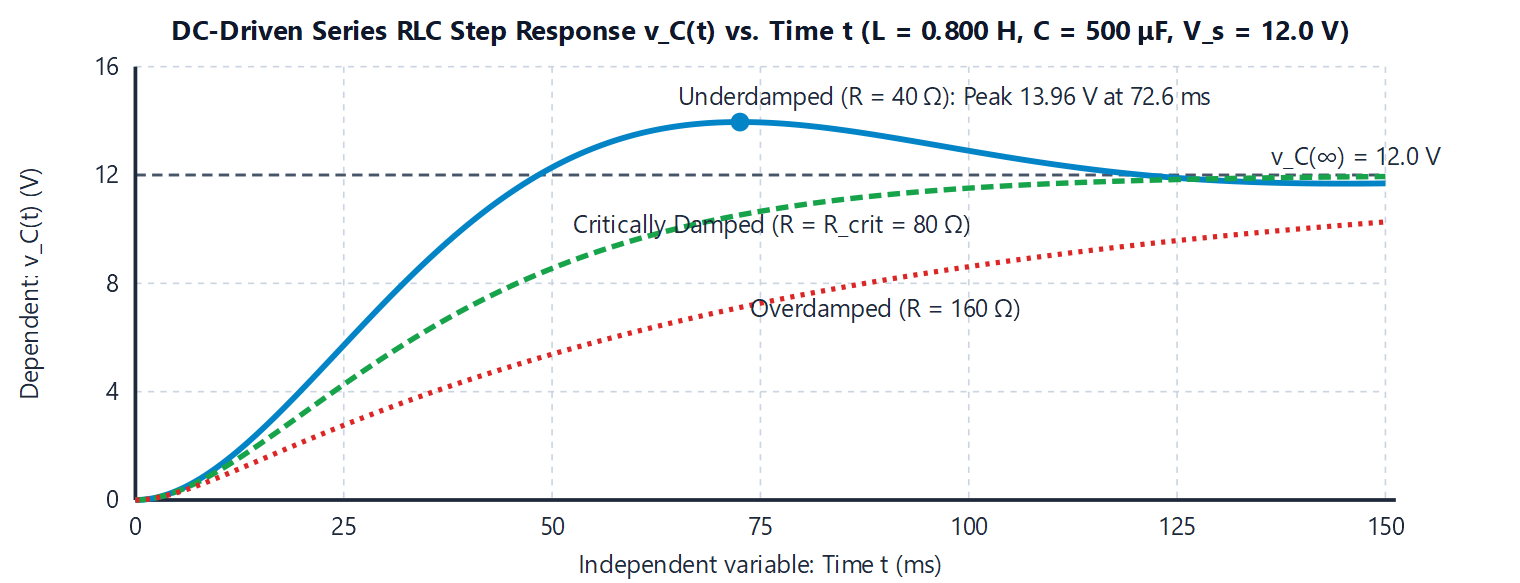
\includegraphics[width=0.82\linewidth]{day1_assets/s4-q3-grid-solved.png}\end{center}

\end{document}
